\documentclass[a4paper,twoside]{article}
\usepackage{blindtext}  
\usepackage{geometry}

% Chinese support
\usepackage[UTF8, scheme = plain]{ctex}

% Page margin layout
\geometry{left=2.3cm,right=2cm,top=2.5cm,bottom=2.0cm}


\usepackage{listings}
\usepackage{xcolor}
\usepackage{geometry}
\usepackage{amsmath}
\usepackage{float}
\usepackage{hyperref}

\usepackage{graphics}
\usepackage{graphicx}
\usepackage{epsfig}
\usepackage{float}
\usepackage{wrapfig}

\usepackage{algorithm}
\usepackage[noend]{algpseudocode}

\usepackage{booktabs}
\usepackage{threeparttable}
\usepackage{longtable}
\usepackage{listings}
\usepackage{tikz}
\usepackage{multicol}

\usepackage{caption}
\usepackage{subcaption}

% cite package, to clean up citations in the main text. Do not remove.
\usepackage{cite}

\usepackage{color,xcolor}

%% The amssymb package provides various useful mathematical symbols
\usepackage{amssymb}
%% The amsthm package provides extended theorem environments
\usepackage{amsthm}
\usepackage{amsfonts}
\usepackage{enumerate}
\usepackage{enumitem}
\usepackage{listings}

\usepackage{textcomp}

\usepackage{indentfirst}
\setlength{\parindent}{2em} % Make two letter space in the first paragraph
\usepackage{setspace}
\linespread{1.5} % Line spacing setting
\usepackage{siunitx}
\setlength{\parskip}{0.5em} % Paragraph spacing setting

% \usepackage[contents =22920202204622, scale = 10, color = black, angle = 50, opacity = .10]{background}

\renewcommand{\figurename}{图}
\renewcommand{\lstlistingname}{代码} 
\renewcommand{\tablename}{表格}
\renewcommand{\contentsname}{目录}
\floatname{algorithm}{算法}

\graphicspath{ {images/} }

%%%%%%%%%%%%%
\newcommand{\StudentNumber}{22920202204622}  % Fill your student number here
\newcommand{\StudentName}{熊恪峥}  % Replace your name here
\newcommand{\PaperTitle}{实验(五) 哲学家就餐问题}  % Change your paper title here
\newcommand{\PaperType}{Unix程序设计} % Replace the type of your report here
\newcommand{\Date}{2022年12月10日}
\newcommand{\College}{信息学院}
\newcommand{\CourseName}{Unix程序设计}
%%%%%%%%%%%%%

%% Page header and footer setting
\usepackage{fancyhdr}
\usepackage{lastpage}
\pagestyle{fancy}
\fancyhf{}
% This requires the document to be twoside
\fancyhead[LO]{\texttt{\StudentName }}
\fancyhead[LE]{\texttt{\StudentNumber}}
\fancyhead[C]{\texttt{\PaperTitle }}
\fancyhead[R]{\texttt{第{\thepage}页,共\pageref*{LastPage}页}}


\title{\PaperTitle}
\author{\StudentName}
\date{\Date}

\lstset{
	basicstyle          =   \sffamily,          % 基本代码风格
	keywordstyle        =   \bfseries,          % 关键字风格
	commentstyle        =   \rmfamily\itshape,  % 注释的风格,斜体
	stringstyle         =   \ttfamily,  % 字符串风格
	flexiblecolumns,                % 别问为什么,加上这个
	numbers             =   left,   % 行号的位置在左边
	showspaces          =   false,  % 是否显示空格,显示了有点乱,所以不现实了
	numberstyle         =   \zihao{-5}\ttfamily,    % 行号的样式,小五号,tt等宽字体
	showstringspaces    =   false,
	captionpos          =   t,      % 这段代码的名字所呈现的位置,t指的是top上面
	frame               =   lrtb,   % 显示边框
}

\lstdefinestyle{PythonStyle}{
	language        =   Python, % 语言选Python
	basicstyle      =   \zihao{-5}\ttfamily,
	numberstyle     =   \zihao{-5}\ttfamily,
	keywordstyle    =   \color{blue},
	keywordstyle    =   [2] \color{teal},
	stringstyle     =   \color{magenta},
	commentstyle    =   \color{red}\ttfamily,
	breaklines      =   true,   % 自动换行,建议不要写太长的行
	columns         =   fixed,  % 如果不加这一句,字间距就不固定,很丑,必须加
	basewidth       =   0.5em,
}

\definecolor{keycolor}{RGB}{172, 42, 42}
\definecolor{mbleu}{RGB}{64,96,127}
\definecolor{vimvert}{RGB}{46, 139, 87}

\lstdefinestyle{MakefileBaseStyle}{
basicstyle=\ttfamily\scriptsize\color{black!90},%
stringstyle=\itshape\color{magenta},%
showstringspaces=false,%
keywordstyle=\bfseries\color{keycolor},%
commentstyle=\color{blue}\slshape,%
framexleftmargin=1mm,%
backgroundcolor=\color{black!2},%
}

\lstdefinestyle{MakefileStyle}{
	otherkeywords={.SUFFIXES},
	morekeywords={SUFFIX, CPP_,},
	moredelim=[is][\color{mbleu}]{/*}{*/},
	style=MakefileBaseStyle,%
	morecomment=[l][commentstyle]{\#},%
	emphstyle={\color{vimvert}},%
	moredelim=[s][\color{vimvert}]{\$(}{)}%
}

\lstdefinestyle{CppStyle}{
	language        =   c++,
	basicstyle      =   \zihao{-5}\ttfamily,
	numberstyle     =   \zihao{-5}\ttfamily,
	keywordstyle    =   \color{blue},
	keywordstyle    =   [2] \color{teal},
	stringstyle     =   \color{magenta},
	commentstyle    =   \color{red}\ttfamily,
	breaklines      =   true,   % 自动换行,建议不要写太长的行
	columns         =   fixed,  % 如果不加这一句,字间距就不固定,很丑,必须加
	basewidth       =   0.5em,
}

\algnewcommand\algorithmicinput{\textbf{Input:}}
\algnewcommand\algorithmicoutput{\textbf{Output:}}
\algnewcommand\Input{\item[\algorithmicinput]}%
\algnewcommand\Output{\item[\algorithmicoutput]}%

\usetikzlibrary{positioning, shapes.geometric}

% 流程图定义基本形状
\tikzstyle{startstop} = [rectangle, rounded corners, minimum width = 2cm, minimum height=1cm,text centered, draw = black]
\tikzstyle{io} = [trapezium, trapezium left angle=70, trapezium right angle=110, minimum width=2cm, minimum height=1cm, text centered, draw=black]
\tikzstyle{process} = [rectangle, minimum width=3cm, minimum height=1cm, text centered, draw=black]
\tikzstyle{decision} = [diamond, aspect = 3, text centered, draw=black]
% 箭头形式
\tikzstyle{arrow} = [->,>=stealth]

\newtheorem{assumption}{Assumption}[section]

\begin{document}
	
%%%%%%%%%%%%%%%%%%%%%%%%%%%%%%%%%%%%%%%%%%%%
\makeatletter % change default title style
\renewcommand*\maketitle{%
	\begin{center} 
		\bfseries  % title 
		{\LARGE \@title \par}  % LARGE typesetting
		\vskip 1em  %  margin 1em
		{\global\let\author\@empty}  % no author information
		{\global\let\date\@empty}  % no date
		\thispagestyle{empty}   %  empty page style
	\end{center}%
	\setcounter{footnote}{0}%
}
\makeatother
%%%%%%%%%%%%%%%%%%%%%%%%%%%%%%%%%%%%%%%%%%%%
	
	
\thispagestyle{empty}

\vspace*{1cm}

\begin{figure}[h]
	\centering
	
\includegraphics[width=4.0cm]{logo.png}
\end{figure}

\vspace*{1cm}

\begin{center}
	\Huge{\textbf{\PaperType}}
	
	\Large{\PaperTitle}
\end{center}

\vspace*{1cm}

\begin{table}[h]
	\centering	
	\begin{Large}
		\renewcommand{\arraystretch}{1.5}
		\begin{tabular}{p{3cm} p{5cm}<{\centering}}
			姓\qquad 名 & \StudentName  \\
			\hline
			学\qquad号 & \StudentNumber \\
			\hline
			日\qquad期 & \Date  \\
			\hline
			学\qquad院 & \College  \\
			\hline
			课程名称 & \CourseName  \\
			\hline
		\end{tabular}
	\end{Large}
\end{table}

\newpage

\title{
	\Large{\textcolor{black}{\PaperTitle}}
}
	
	
\maketitle
	
\tableofcontents
 
\newpage
\setcounter{page}{1}

\begin{spacing}{1.2}

\section{实验内容}

编制模拟“五个哲学家”问题的程序。程序语法:
\begin{center}
	\texttt{philosopher   [ -t  \textless time \textgreater ]	}
\end{center}
\textless time \textgreater是哲学家进餐和沉思的持续时间值,缺省值为2秒。
\begin{enumerate}
    \item 五个哲学家的编号为$0\cdots4$,分别用五个进程独立模拟。
	\item 程序的输出要简洁,仅输出每个哲学家进餐和沉思的信息。例如,当编号为3的哲学家在进餐时,就打印:philosopher 3 is eating。而当他在沉思时,则打印:philosopher 3 is thinking。除此之外不要输出其他任何信息。
\end{enumerate}

\section{使用文件同步的实现}

哲学家就餐问题是一种用于描述资源同步和解决方案的问题\cite{wiki:dpp}。
该问题描述了五个哲学家围坐在一张圆桌周围,每个哲学家面前都有一碗饭和一根筷子。哲学家们的生活方式是交替地思考和进餐,思考时不使用筷子,
进餐时需要使用两根筷子。当一个哲学家进餐时,他需要同时拿起左右两边的筷子,如果两边的筷子都被其他哲学家拿着,
那么他就需要等待,直到两边的筷子都空闲下来。当一个哲学家拿起一根筷子时,他就会把它放在桌子上,以示其他哲学家可以拿起它。
当一个哲学家进餐完毕,他会把两根筷子放回桌子上,然后开始思考\cite{wiki:Dining_philosophers_problem},如图~\ref{fig:philosopher}所示。
\footnote{图片:\url{https://en.wikipedia.org/wiki/Dining_philosophers_problem}}

\begin{figure}[h]
	\centering
	\caption{哲学家就餐问题}
	\label{fig:philosopher}
	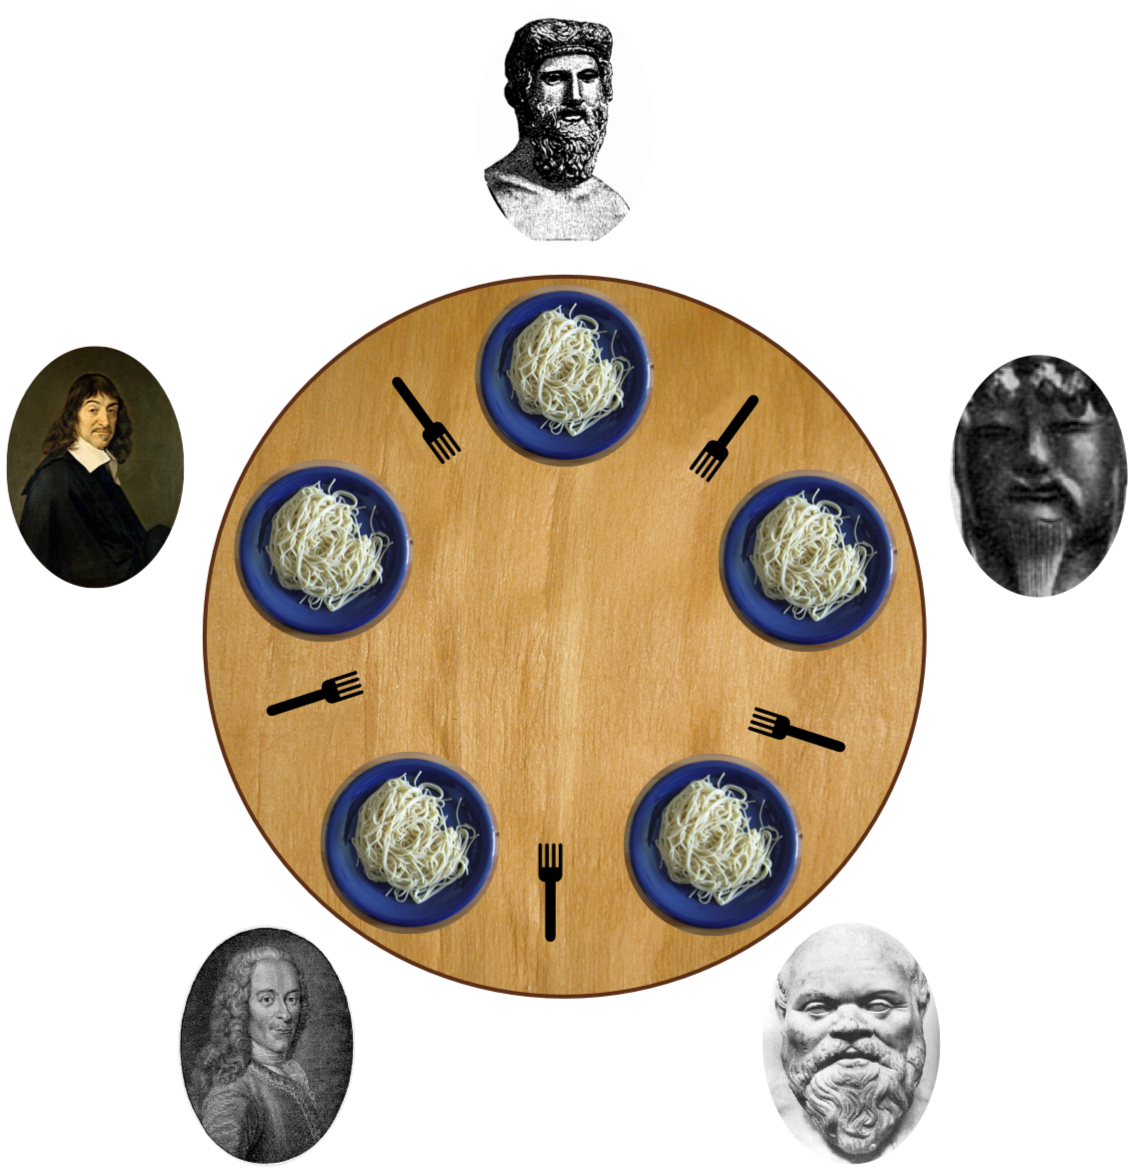
\includegraphics[width=0.4\textwidth]{philosopher.png}
\end{figure}

为了实现同步,有多种可以考虑的方法。使用文件是一种简单直接地方法。\texttt{lock.c}通过文件实现了一种互斥锁。
如\nameref{sec:code}中的代码~\ref{code:lock}所示。为了获取锁,程序就会使用\texttt{O\_EXCL}标志
尝试创建对应的文件。如果此时已经有进程拥有这把锁,就会导致创建失败,因此尝试获取锁的进程就会休眠一段时间
再试。这样就实现了互斥锁的效果。为了释放锁,进程只需要删除对应的文件即可。

使用这种互斥锁的方法,可以实现哲学家就餐问题。如\nameref{sec:code}中的代码~\ref{code:phi1}所示。
在这个程序中,每个哲学家都是一个进程,每个进程都会尝试获取左右两边的筷子,如果获取成功,就会进餐。
在这个实现中,解决死锁问题的方法是“指定一个哲学家,它获取两把筷子的顺序和其他人相反。”。这种方法本质上
是一种“资源分级”的解决方案。它相当于给筷子A、B、C、D、E赋予优先级,然后要求各哲学家都先获取优先级低的筷子,
再获取优先级高的筷子。这样就可以避免死锁的发生。

这种方法能够避免死锁发生,但它不是公平的。尤其是当哲学家思考的时间不同的时候,可能思考时间较长的哲学家
永远没有办法进餐。此外,利用文件实现互斥锁的方法也有一些缺点。首先,它需要创建文件,这样就会占用磁盘空间。
文件I/O也是一种引入了额外开销的操作。

为了解决后者的问题,可以使用\textbf{信号量}。

\section{使用信号量优化上述实现}

信号量(Semaphores)是一种常见的同步原语(Primitives)。信号量是一个变量或者抽象数据类型,它的作用是用来控制多个线程或进程对共享资源的访问,
避免并行系统中的关键资源被多个进程同时访问而导致的不一致性。信号量的值是一个非负整数,它可以表示共享资源的数量。POSIX API提供了
创建可以在进程间共享的信号量的方法。

信号量的基本操作可以被称为P操作和V操作。P操作是“等待”操作,它会使信号量的值减1。如果信号量的值为0,那么P操作会使进程休眠,
直到信号量的值大于0。V操作是“释放”操作,它会使信号量的值加1。如果有进程在等待信号量,那么V操作会唤醒一个等待进程。对应的POSIX API
如表~\ref{tbl:sem}所示。

\begin{table}[htbp]
	\centering
	\caption{信号量的POSIX API}
	\label{tbl:sem}
	\begin{tabular}{c|c|c}
		\toprule
		\hline
		\textbf{函数} & \textbf{功能} & \textbf{返回值} \\
		\hline
		sem\_init & 初始化信号量 & 0 \\
		\hline
		sem\_wait & P操作 & 0 \\
		\hline
		sem\_post & V操作 & 0 \\
		\hline
		sem\_destroy & 销毁信号量 & 0 \\
		\hline
		\bottomrule
	\end{tabular}
\end{table}

使用信号量的实现如\nameref{sec:code}中的代码~\ref{code:sem}所示。

\section{另一种解决方案}

除了限定哲学家中同时存在左撇子和右撇子,还可以通过限制能吃饭的哲学家的数量来避免死锁\cite{stallings2012operating}。这种方法的思路是,当有哲学家想要进餐的时候,
需要进入“餐厅”,餐厅仅限4个人,这样每人都有足够的叉子。如果餐厅已经满了,那么哲学家就需要等待。当有哲学家离开餐厅的时候,餐厅就会有空位,这时候可以让等待的哲学家进入餐厅。

这样,就可以用初始值为4的信号量来表示餐厅的空位数。当哲学家想要进入餐厅的时候,就需要执行P操作,如果餐厅有空位,那么P操作就会成功,哲学家就可以进入餐厅。当哲学家离开餐厅的时候,就需要执行V操作,这样餐厅的空位数就会加1,可以让等待的哲学家进入餐厅。

这样的实现如\nameref{sec:code}中的代码~\ref{code:sem2}所示。

\section{运行效果}

以上三种实现的运行效果都大致如图~\ref{fig:res}所示。
\begin{figure}[h]
	\centering
	\caption{哲学家就餐问题}
	\label{fig:res}
	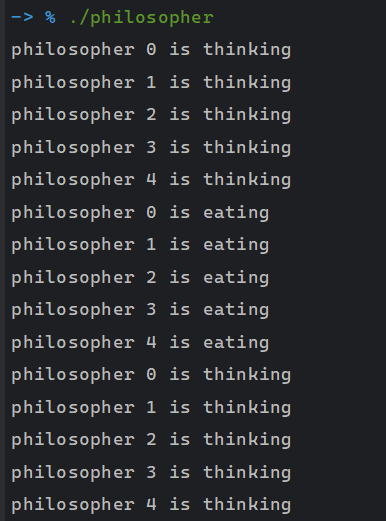
\includegraphics[width=0.4\textwidth]{res.png}
\end{figure}
可见,所有哲学家都能正常进餐,这些实现都是正确的。

\section{实验总结}

本次实现通过解决哲学家就餐问题,让我了解到了多进程同步的基本概念和方法。
通过本次实验,我学会了使用文件和信号量来实现进程同步,并解决哲学家就餐问题。
了解到了在并发的系统中保护Critical Section的基本方法。

\appendix

\clearpage
\section*{参考文献}
\addcontentsline{toc}{part}{参考文献}

\bibliographystyle{unsrt}
\bibliography{reference}

\clearpage
\section*{附录:代码清单}
\addcontentsline{toc}{part}{附录:代码清单}
\label{sec:code}

\begin{lstlisting}[numbers=left,style=CppStyle,caption=\texttt{lock.c},label={code:lock}]
#include	<sys/types.h>
#include	<sys/stat.h>
#include	<fcntl.h>
#include	<unistd.h>
#include	"apue.h"

void initlock(const char *lockfile)
{
	int	i;

	unlink(lockfile);
}

void lock(const char *lockfile)
{
	int	fd;
	while ( (fd = open(lockfile, O_RDONLY | O_CREAT | O_EXCL, FILE_MODE)) < 0)
		sleep(1);
	close(fd);
}

void unlock(const char *lockfile)
{
	unlink(lockfile);
}
\end{lstlisting}

\begin{lstlisting}[numbers=left,style=CppStyle,caption=使用文件实现,label={code:phi1}]
//
// Created by bear on 12/3/2022.
//
#include "apue.h"
#include "lock.h"
#include "error.h"

#include "sys/wait.h"

#define N 5

static char *forks[5] = {"fork0", "fork1", "fork2", "fork3", "fork4"};

void putFork(int i)
{
	if (i == N - 1)
	{
		unlock(forks[0]);
		unlock(forks[i]);
	}
	else
	{
		unlock(forks[i]);
		unlock(forks[i + 1]);
	}
}

void takeFork(int i)
{
	if (i == N - 1)
	{
		lock(forks[0]);
		lock(forks[i]);
	}
	else
	{
		lock(forks[i]);
		lock(forks[i + 1]);
	}
}

void eating(int i, int nsecs)
{
	printf("philosopher %d is eating\n", i);
	sleep(nsecs);
}

void thinking(int i, int nsecs)
{
	printf("philosopher %d is thinking\n", i);
	sleep(nsecs);
}

void philosopher(int i, int nsecs)
{
	for (;;)
	{
		thinking(i, nsecs);
		takeFork(i);
		eating(i, nsecs);
		putFork(i);
	}
}

int main(int argc, char **argv)
{
	int nsecs = 0;
	if (argc != 3 && argc != 1)
	{
		printf("usage: %s [-t <nsecs>]", argv[0]);
	}

	if (strcmp(argv[2], "-t") == 0)
	{
		nsecs = atoi(argv[3]);
	}
	else
	{
		nsecs = 2;
	}

	for (int i = 0; i < N; i++)
	{
		pid_t pid = fork();
		if (pid == 0)
		{
			philosopher(i, nsecs);
		}
	}

	wait(NULL);
	return 0;
}
\end{lstlisting}

\begin{lstlisting}[numbers=left,style=CppStyle,caption=使用信号量实现,label={code:sem}]
#define N 5

static sem_t forks_sems[5];

void init_sems()
{
	for (int i = 0; i < N; i++)
	{
		if (sem_init(&forks_sems[i], 1, 1) != 0)
		{
			err_sys("sem_open error");
		}
	}
}

void destroy_sems()
{
	for (int i = 0; i < N; i++)
	{
		sem_destroy(&forks_sems[i]);
	}
}

void putFork(int i)
{
	if (i == N - 1)
	{
		sem_post(&forks_sems[0]);
		sem_post(&forks_sems[i]);
	}
	else
	{
		sem_post(&forks_sems[i]);
		sem_post(&forks_sems[i + 1]);
	}
}

void takeFork(int i)
{
	if (i == N - 1)
	{
		sem_wait(&forks_sems[0]);
		sem_wait(&forks_sems[i]);
	}
	else
	{
		sem_wait(&forks_sems[i]);
		sem_wait(&forks_sems[i + 1]);
	}
}

void eating(int i, int nsecs)
{
	printf("philosopher %d is eating\n", i);
	sleep(nsecs);
}

void thinking(int i, int nsecs)
{
	printf("philosopher %d is thinking\n", i);
	sleep(nsecs);
}

void philosopher(int i, int nsecs)
{
	for (;;)
	{
		thinking(i, nsecs);
		takeFork(i);
		eating(i, nsecs);
		putFork(i);
	}
}
\end{lstlisting}

\begin{lstlisting}[numbers=left,style=CppStyle,caption=另一种实现,label={code:sem2}]
	#define N 5

static sem_t forks_sems[5];
static sem_t room_sem;

void init_sems()
{
	sem_init(&room_sem, 1, N - 1);
	for (int i = 0; i < N; i++)
	{
		if (sem_init(&forks_sems[i], 1, 1) != 0)
		{
			err_sys("sem_open error");
		}
	}
}

void destroy_sems()
{
	sem_destroy(&room_sem);
	for (int i = 0; i < N; i++)
	{
		sem_destroy(&forks_sems[i]);
	}
}

void putFork(int i)
{
	if (i == N - 1)
	{
		sem_post(&forks_sems[0]);
		sem_post(&forks_sems[i]);
	}
	else
	{
		sem_post(&forks_sems[i]);
		sem_post(&forks_sems[i + 1]);
	}
}

void takeFork(int i)
{
	if (i == N - 1)
	{
		sem_wait(&forks_sems[0]);
		sem_wait(&forks_sems[i]);
	}
	else
	{
		sem_wait(&forks_sems[i]);
		sem_wait(&forks_sems[i + 1]);
	}
}

void eating(int i, int nsecs)
{
	printf("philosopher %d is eating\n", i);
	sleep(nsecs);
}

void thinking(int i, int nsecs)
{
	printf("philosopher %d is thinking\n", i);
	sleep(nsecs);
}

void philosopher(int i, int nsecs)
{
	for (;;)
	{
		thinking(i, nsecs);
		sem_wait(&room_sem);
		takeFork(i);
		eating(i, nsecs);
		putFork(i);
		sem_post(&room_sem);
	}
}
\end{lstlisting}


\end{spacing}

\end{document}